% Source: Wald GR, physical PDF p. 418
%         (printed p. 405).
% Coverage: Backward propagation through collapsing matter.
% Figures/tables/footnotes: Figure 14.3; no tables or footnotes.
% Status: source-reviewed and compile-clean.
% Uncertainties: none.

\begingroup
\renewcommand{\thefigure}{14.3}
\begin{figure}[htbp]
  \centering
  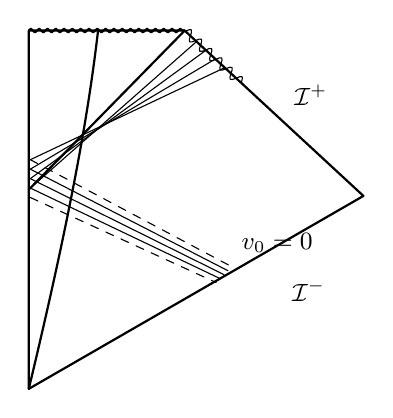
\begin{tikzpicture}[x=1cm,y=1cm,font=\small,line cap=round,line join=round]
    \coordinate (B) at (-1.70,-2.35);
    \coordinate (A) at (-1.70,2.20);
    \coordinate (S) at (.28,2.20);
    \coordinate (R) at (2.55,.10);
    \draw[thick] (B)--(A)--(S)--(R)--cycle;
    \draw[thick,decorate,decoration={zigzag,segment length=3pt,amplitude=.65pt}]
      (A)--(S);
    % Surface of the collapsing body and event horizon.
    \draw[thick] (B) .. controls (-1.10,.15) and (-.92,1.35) .. (-.82,2.20);
    \draw[thick] (-1.70,.18)--(S);
    % Backward-propagated wave fronts.  The upper family arrives from
    % \mathcal I^+; its continuation through the collapsing body accumulates
    % at the point v_0=0 on \mathcal I^-.
    \draw[thin] (-1.68,.20)--(.43,2.06);
    \draw[thin] (-1.68,.32)--(.55,1.95);
    \draw[thin] (-1.68,.44)--(.67,1.84);
    \draw[thin] (-1.68,.56)--(.79,1.73);
    \draw[thin] (-1.68,.20)--(.73,-.95);
    \draw[thin] (-1.68,.32)--(.78,-.90);
    \draw[thin] (-1.68,.44)--(.83,-.85);
    \draw[dashed] (-1.68,.08)--(.68,-1.00);
    \draw[dashed] (-1.68,.56)--(.88,-.80);
    \node[anchor=south west] at (.88,-.74) {\(v_0=0\)};
    \node[right] at (1.55,1.38) {\(\mathcal I^+\)};
    \node[right] at (1.52,-1.10) {\(\mathcal I^-\)};
    \draw[decorate,decoration={snake,segment length=5pt,amplitude=1.8pt}]
      (S)--(1.05,1.49);
  \end{tikzpicture}
  \caption{A conformal diagram of a spherically symmetric spacetime in which
  gravitational collapse to a Schwarzschild black hole occurs, showing the
  oscillations of a wave which behaves as \(e^{-\ii\omega u}\) on
  \(\mathcal I^+\). If one propagates this wave backward into the past starting
  from \(\mathcal I^+\), the part of the wave which propagates through the
  collapsing matter will produce an ``infinite blueshift'' singularity---of the same
  nature as shown on the white hole horizon in Figure~\ref{fig:14.2}---at advanced
  time \(v_0\) on \(\mathcal I^-\).}
  \label{fig:14.3}
\end{figure}
\endgroup
